% coding:utf-8
\section{Stammfunktion}
a)\\
$x<0$: Steigung negativ\\
$x=0$: Steigung null\\
$x<0$ Steigung positiv\\\\
b)\\
$e^x$ ist abgeleitet sich selbst. $e^{-x}$ ist abgeleitet $-e^{-x}$. 

\section{Autofahrt}
\[ v(t) = a t^3 - b t^2 + c t \]
\[ s(t) = \int (v(t)) dt = \underline{\underline{\frac{a t^4}{4} - \frac{b t^3}{3} + \frac{c t^2}{2}}} \]

\section{Schwimmbecken}
\[ v(t) = a \cdot e^{-bt} \]
\[ V(t) = \int v(t) dt = \int \left(a \cdot e^{-bt}\right) dt = -\frac{a \cdot e^{-bt}}{b} + c \]
c ist die Integrationskonstante
\[ V(0) = 0 \]
\[ -\frac{a \cdot e^{0}}{b} + c = 0 \]
\[ -\frac{a}{b} + c = 0 \]
\[ c = \frac{a}{b} \]
\[ \rightarrow V(t) = -\frac{a \cdot e^{-bt}}{b} + \frac{a}{b} = -\frac{a}{b} \left( e^{-bt} - 1 \right) \]
\[ -V(t) \cdot \frac{b}{a} = e^{-bt} - 1 \]
\[ -V(t) \cdot \frac{b}{a} + 1 = e^{-bt} \]
\[ -bt = \ln\left(-V(t) \cdot \frac{b}{a} + 1\right) \]
\[ \underline{\underline{t = -\frac{\ln\left(-V(t) \cdot \frac{b}{a} + 1\right)}{b}}} \]

\section{Fläche durch Tangente}
\[ f(x) = x^3 + x^2 \]
\[ f'(x) = 3 x^2 + 2 x \]
\[ T(x) = f'(x_0)(x - x_0) + f(x_0) \]
\[ T(x) = (3 {x_0}^3 + 2 x_0)(x-x_0) + {x_0}^3 + {x_0}^2 \]
\[ T(x) = 3 x {x_0}^2 - 3 {x_0}^3 + 2 x x_0 - 2 {x_0}^2 + {x_0}^3 + {x_0}^2 \]
\[ T(x) = 3 x {x_0}^2 - 2 {x_0}^3 + 2 x x_0 - {x_0}^2 \]
\[ T(x) = x(3 {x_0}^2 + 2 x_0) - (2 {x_0}^3 + {x_0}^2) \]
\[ T(x) = 0 \]
\[ x_1 = \frac{2 {x_0}^3 + {x_0}^2}{3 {x_0}^2 + 2 x_0} \]
\[ A = A_{Gesamt} - A_\Delta \]
\[ A_\Delta = \frac{(x_0 - x_1) \cdot f(x_0)}{2} = \frac{(x_0 - x_1) \cdot ({x_0}^3 + {x_0}^2)}{2} \]
\[ A_{Gesamt} = \int_0^{x_0} (x^3 + x^2) dx = \left.\frac{x^4}{4} + \frac{x^3}{3} \right|_{0}^{x_0} = \frac{{x_0}^4}{4} + \frac{{x_0}^3}{3} \]
\[ A = A_{Gesamt} - A_\Delta = \underline{\underline{\frac{{x_0}^4}{4} + \frac{{x_0}^3}{3} - \frac{(x_0 - x_1) \cdot ({x_0}^3 + {x_0}^2)}{2}}} = -\frac{{x_0}^4}{4} + \frac{5 {x_0}^3}{6} - \frac{x_1 ({x_0}^3 + {x_0}^2)}{2} \]

\section{Eingeschlossener Flächeninhalt}
Aufgabenstellung: 
\[ f(x) = ax^2 - bax \]
\[ g(x) = ax \]
\[ a < 0 \]
Lösung: 
\[ f(x_0) = g(x_0) \quad x_0 \neq 0 \]
\[ a{x_0}^2 - bax_0 = ax_0 \]
\[ a{x_0}^2 - (b+1)ax_0 = 0 \]
\[ x_{0_{1,2}} = \frac{(b+1)a \pm \sqrt{(b+1)^2a^2}}{2a} = \frac{b+1)a \pm (b+1)a}{2a} = \frac{(b+1) \pm (b+1)}{2} \]
\[ x_{0_1} = \frac{2(b+1)}{2} = b+1 \]
\[ x_{0_2} = \frac{0}{2} = 0 \quad \Rightarrow \text{keine Lösung} \]
\[ F(x) = \int_0^{x_0} (ax^2 - (b+1)ax) dx = \left.\frac{ax^3}{3} - \frac{b(a+1)x^2}{2}\right|_0^{x_0} = \frac{a{x_0}^3}{3} - \frac{(b+1)a{x_0}^2}{2} \]
\[ = \frac{a{(b+1)}^3}{3} - \frac{a{(b+1)}^3}{2} = \frac{2a(b+1)^3}{6} - \frac{3a(b+1)^3}{6} = -\frac{a(b+1)^3}{6} \]
\[ \Rightarrow \underline{\underline{a = -\frac{6F}{(b+1)^3}}} \]

\section{Horizontale Linie}
\[ f(x) = x^2 \]
\[ g(x) = y_0 \]
\[ f^{-1}(y) = \sqrt{y} \]
\[ F_1 = \int_{y_1}^{y_0} f^{-1}(y) dy = \int_{y_1}^{y_0} \left(\sqrt{y}\right) dy = \left.\frac{2}{3} y^{\frac{3}{2}}\right|_{y_1}^{y_0} = \frac{2}{3}{y_0}^{\frac{3}{2}} - \frac{2}{3}{y_1}^{\frac{3}{2}} \]
\[ F_2 = \int_{0}^{y_1} f^{-1}(y) dy = \int_{0}^{y_1} \left(\sqrt{y}\right) dy = \left.\frac{2}{3} y^{\frac{3}{2}}\right|_{0}^{y_1} = \frac{2}{3}{y_1}^{\frac{3}{2}} \]
\[ F_1 = F_2 \]
\[ \frac{2}{3}{y_0}^{\frac{3}{2}} - \frac{2}{3}{y_1}^{\frac{3}{2}} = \frac{2}{3}{y_1}^{\frac{3}{2}} \]
\[ \frac{2}{3}{y_0}^{\frac{3}{2}} = \frac{4}{3}{y_1}^{\frac{3}{2}} \]
\[ {y_0}^{\frac{3}{2}} = 2 \cdot {y_1}^{\frac{3}{2}} \]
\[ \frac{{y_0}^{\frac{3}{2}}}{2} = {y_1}^{\frac{3}{2}} \]
\[ y_1 = \underline{\underline{\frac{y_0}{2^{\frac{2}{3}}} \approx \frac{y_0}{1.5874}}} \]

\section{Vase}
\[ f(x) = \sqrt{x+a} \]
\[ g(x) = \sqrt{x-b} \]
\[ V(x) = \pi \int_0^h f(x)^2 dx - \pi \int_b^h g(x)^2dx = \pi \left( \int_0^h (x+a) dx - \int_b^h (x-b) dx\right) \]
a)
\[ V(x) = \pi\left(\left. \frac{h^2}{2} + ah \right|_0^h - \left(\left. \frac{x^2}{2} - bx \right|_b^h \right) \right) = \pi \left(  \frac{h^2}{2} + ah - \left( \frac{h^2}{2} - bh - \frac{b^2}{b} + b^2 \right)\right) \]
\[ = \pi \left(\frac{h^2}{2} + ah - \frac{h^2}{2} + bh + \frac{b^2}{2} - b^2\right) = \pi \left(ah + bh + \frac{b^2}{2} - b^2\right) \]
\[ V(x) = \pi \left(ah + bh - b^2\right) \]
\[ \Rightarrow \underline{\underline{m = V \cdot \rho = \pi \cdot \rho \cdot \left(ah + bh - \frac{b^2}{2}\right)}} \]
b)
\[ A_{M_x} = 2 \pi \int_0^h f(x) \sqrt{1 + f'(x)^2} dx \]
\[ A_{M_x} = 2 \pi \int_0^h \sqrt{x + a} \cdot \sqrt{1 + \left( \frac{1}{2 \sqrt{x + a}} \right)^2} dx \]
\[ A_{M_x} = 2 \pi \int_0^h \sqrt{(x + a) \cdot \left(1 + \frac{1}{4 (x + a)} \right)} dx \]
\[ A_{M_x} = 2 \pi \int_0^h \sqrt{x + a + \frac{1}{4}} dx \]
\[ A_{M_x} = 2 \pi \int_0^h \frac{1}{2} \sqrt{4x + 4a + 1} dx \]
\[ A_{M_x} = \left. 2 \pi \cdot \frac{1}{2} \frac{2}{3}\left( 4x + 4a + 1 \right)^{\frac{3}{2}} \cdot \frac{1}{4} \right|_0^h \]
\[ A_{M_x} = \left. \frac{1}{6} \pi \left(4x + 4a + 1\right)^{\frac{3}{2}} \right|_0^h \]
\[ \rightarrow A_{M_x} = \frac{1}{6} \pi \left(\left( 4h + 4a + 1 \right)^{\frac{3}{2}} - \left(4a + 1\right)^{\frac{3}{2}}\right) \]
\[ A_B = f(0)^2 \cdot \pi = a \pi \]
\[ A_D = f(h)^2 \cdot \pi - g(h)^2 \cdot \pi = \pi \left( f(h)^2 - g(h)^2 \right) = \pi \left( h + a - h + b \right) = \pi \left( a + b \right) \]
\[ A =  A_{M_x} + A_B + A_D = \frac{1}{6} \pi \left(\left( 4h + 4a + 1 \right)^{\frac{3}{2}} - \left(4a + 1\right)^{\frac{3}{2}}\right) + a \pi + \pi \left( a + b \right) \]
\[ A =  A_{M_x} + A_B + A_D = \pi \left(\frac{1}{6} \left(\left( 4h + 4a + 1 \right)^{\frac{3}{2}} - \left(4a + 1\right)^{\frac{3}{2}}\right) + a + \left( a + b \right)\right) \]
\[ \underline{\underline{A =  A_{M_x} + A_B + A_D = \pi \left(\frac{1}{6} \left(\left( 4h + 4a + 1 \right)^{\frac{3}{2}} - \left(4a + 1\right)^{\frac{3}{2}}\right) + 2a + b\right)}} \]

\section{Zykloide}
\[  \]

\section{Fahrzeug}
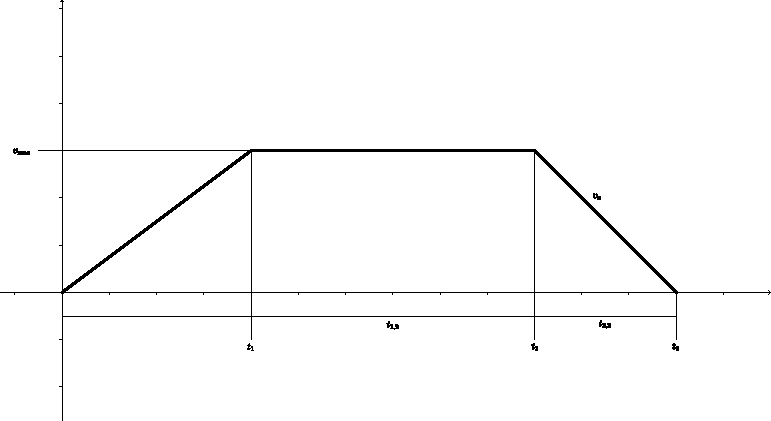
\includegraphics[width=0.8\textwidth]{bilder/fahrzeug_svg.pdf}
a)
\[ s = s_1 + s_2 + s_3 \]
\[ s_1 = \int_0^{t_1} v(t) dt = \int_0^{t_1} \left( \frac{v_{max}}{t_1} \cdot t \right) dt = \left. \frac{v_{max} \cdot t^2}{2 t_1} \right|_0^{t_1} = \frac{v_{max} \cdot {t_1}^2}{2 t_1} = \frac{v_{max} \cdot {t_1}}{2} \]
\[ s_2 = \int_{t_1}^{t_2} v_{max} dt = t_2 \cdot v_{max} - t_1 \cdot v_{max} = v_{max} \cdot (t_2 - t_1) = v_{max} \cdot t_{1,2} \]
\[ s_3 = \int_{t_2}^{t_3} \left(-\frac{v_{max}}{t_{2,3}} \cdot (t - t_{0,1} - t_{1,2} - t_{2,3})\right) dt = \int_{t_2}^{t_3} \left(-\frac{v_{max}}{t_{2,3}} \cdot (t - t_{0,3})\right) dt \]
\[ s_3 = -\frac{v_{max}}{t_{2,3}} \cdot \int_{t_2}^{t_3} \left(t - t_3\right) dt = -\frac{v_{max}}{t_{2,3}} \cdot \left.\left(\frac{t^2}{2} - t \cdot t_3\right)\right|_{t_2}^{t_3} \]
\[ s_3 = -\frac{v_{max}}{t_{2,3}} \cdot \left(\frac{{t_3}^2}{2} - {t_3}^2 - \frac{{t_2}^2}{2} + t_2 \cdot t_3\right) = -\frac{v_{max}}{t_{2,3}} \cdot \left(-\frac{{t_3}^2}{2} - \frac{{t_2}^2}{2} + t_2 \cdot t_3\right) \]
\[ s_3 = -\frac{v_{max}}{t_{2,3}} \cdot \left(-\frac{(t_{2,3} - t_2)^2}{2} - \frac{{t_2}^2}{2} + t_2 \cdot (t_{2,3} - t_2)\right) \]
\[ s_3 = -\frac{v_{max}}{t_{2,3}} \cdot \left(-\frac{{t_{2,3}}^2 - t_{2,3} t_2 + {t_2}^2}{2} - \frac{{t_2}^2}{2} + t_2 t_{2,3} + {t_2}^2\right) \]
\[ s_3 = -\frac{v_{max}}{t_{2,3}} \cdot \left(-\frac{{t_{2,3}}^2}{2} + \frac{t_{2,3} t_2}{2} - \frac{{t_2}^2}{2} - \frac{{t_2}^2}{2} + t_2 t_{2,3} + {t_2}^2\right) \]
\[ s_3 = -\frac{v_{max}}{t_{2,3}} \cdot \left(-\frac{{t_{2,3}}^2}{2} + \frac{t_{2,3} t_2}{2} + t_2 t_{2,3}\right) \]
\[ s_3 = -v_{max} \cdot \left(-\frac{{t_{2,3}}}{2} + \frac{t_2}{2} + t_2\right) \]
Fehler in der Berechnung von $s_3$. Korrekt wäre: 
\[ s_3 = \frac{v_{max} \cdot t_{2,3}}{2} \]
\[ s = s_1 + s_2 + s_3 = \frac{v_{max} \cdot {t_1}}{2} + v_{max} \cdot t_{1,2} + \frac{v_{max} \cdot t_{2,3}}{2} \]
\[ \underline{\underline{s = v_{max} \cdot \left(\frac{{t_1}}{2} + t_{1,2} + \frac{t_{2,3}}{2}\right)}} \]
b)
\[ \underline{\underline{\overline{v} = \frac{s}{t_3} = \frac{s}{t_{1} + t_{1,2} + t_{2,3}}}} \]
c)
\[ v(t_{0_1}) = v(t_{0_2}) = \overline{v} \]
\[ \rightarrow \frac{v_{max}}{t_1} \cdot t_{0_1} = \frac{s}{t_3} \]
\[ \underline{\underline{\Rightarrow t_{0_1} = \frac{s \cdot t_1}{t_3 \cdot v_{max}}}} \]
\[ \rightarrow -\frac{v_{max}}{t_{2,3}} \cdot (t_{0_2} - t_3) = \frac{s}{t_3} \]
\[ t_{0_2} - t_3 = -\frac{s \cdot t_{2,3}}{t_3 \cdot v_{max}} \]
\[ \underline{\underline{\Rightarrow t_{0_2} = -\frac{s \cdot t_{2,3}}{t_3 \cdot v_{max}} + t_3 = -\frac{s \cdot t_{2,3}}{t_3 \cdot v_{max}} + t_1 + t_{1,2} + t_{2,3}}} \]